\section{{Lecture 1 | Intro. to Reinforcement Learning}}

What makes reinfocement learning from other types of learning?
\begin{itemize}
\item There is no supervisor, only a reward signal
\item Feedback is delayed, not instantaneous.
\item Time really matters (sequential, non i.i.d data). Thus, breaks the fundamental assumption of supervised learning.
\item Agent's actions affect the subsequent data it receives. Thus, agent influences the data it receives.
\end{itemize}


Examples of reinforcement learning:
\begin{itemize}
    \item Fly stunt manoeuvres in a helicopter/ or control a robot.
    \item Play backgammon, chess, Go, Atari games.
    \item Manage investment portfolio.
    \item Manage a wind-farm/ power station.
\end{itemize}

\subsection{Elements of Reinforcement Learning --- Rewards}
\begin{itemize}
    \item A reward \(R_t\) is a scalar feedback signal.
    \item Indicates how well agent is doing at step \(t\).
    \item The agent's job is to maximise cumulative reward.
\end{itemize}
The reinforcement learning problem is to maximise the expected cumulative reward. The
reinforcement learning problem is based on the reward hypothesis.
\begin{definition}[Reward Hypothesis]
    All goals can be described by the maximisation of expected cumulative reward.
\end{definition}
Examples of rewards:
\begin{itemize}
    \item Fly stunt manoeuvres in a helicopter/ or control a robot.
    \begin{itemize}
        \item \(R_t = -1 \) for crash
        \item \(R_t = +1\) for following the desired trajectory
    \end{itemize}
    \item Play backgammon, chess, Go, Atari games.
    \begin{itemize}
        \item \(R_t = +1\) for winning the game
        \item \(R_t = 0\) for drawing the game
        \item \(R_t = -1\) for losing the game
    \end{itemize}
\end{itemize}

Sequential Decision Making:
\begin{itemize}
    \item Goal: select actions to maximise total future reward.
    \item Actions may have long term consequences.
    \item Reward may be delayed.
    \item It may be better to sacrifice immediate reward to gain more long-term reward.
    \item Thus, we need to consider the \textbf{whole sequence} of actions and rewards when making a decision.
    \item Examples:
    \begin{itemize}
        \item A financial investment --- may take years to mature.
        \item Refuelling a helicopter --- might prevent a crash in several hours.
        \item Move in chess --- may sacrifice a piece to get an opponent into a position in which they are more likely to lose.
    \end{itemize}
\end{itemize}
\subsection{Elements of Reinforcement Learning --- Agents and Environments}
\begin{figure}[H]
    \centering
    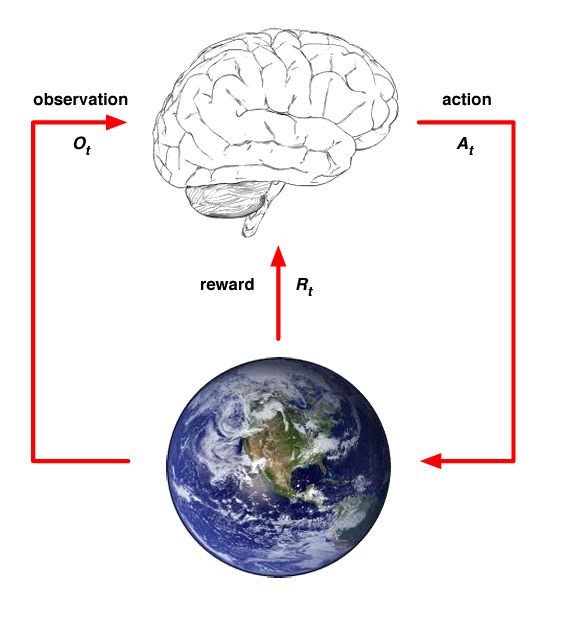
\includegraphics[width=0.60\textwidth]{figures/agent_world.png}
    \caption{Agent and Environment | The RL world loop.}
    \label{fig:agent_world}
\end{figure}

The interaction between the agnet and environments. The brain here represents 
the agent. The goal is to design and build this brain. The agent which take
the actions at each step, based on the information it is receiving from the
environment. The infomation that is coming is usually the observations
and the reward.
Thus, at each step we have for the agent:
\begin{itemize}
    \item The agent executes action \(A_t\).
    \item Receives observation \(O_t\).
    \item Receives scalar reward \(R_t\).
\end{itemize}
And for the environment:
\begin{itemize}
    \item Receives action \(A_t\).
    \item Emits observation \(O_{t+1}\).
    \item Emits scalar reward \(R_{t+1}\).
\end{itemize}

\subsection{Elements of Reinforcement Learning --- State}
History and State:
The history is the sequence of observations, actions, rewards:
\[
    H_t = A_1, O_1, R_1, \dots, A_t, O_t, R_t  
\]
This is practically all the observable variables to the agnet. The environment might have many more
such variables, but the agent does not have access to them. Thus such variables are irrelevant to the
algorithm that the agent will be based on. One of the examples can be the sensorimotor data stream
of the robot.
Ultimately, the agent's choice of action at any given time depends on the history. Thus, what
happens next depends on the history. 
But this history is not very useful. Typically this history is very long, and not practical to
use. Thus, we need to define a more useful quantity, the state.

State: is the information used to determine what happens next. It is the information that is
relevant to make the decision. It is a function of the history:
\[
    S_t = f(H_t)
\]
One of the valid definitions of the state is the complete history, or just the last observation. 
In Atari games, the state is the usually the last 4 frames of the game.

Here we are describing 3 different definations of the state:

Environment State: 
\begin{itemize}
    \item The environment state \(S_t^e\) is the environment's private representation.
    \item whatever the environment uses to pick the next observation and reward. 
    \item The environment state is usually not visible to the agent.
    \item Even if \(S_t^e\) is visible, it may not be useful and might contain irrelevant information.
\end{itemize}

Agent State:
\begin{itemize}
    \item The agent state \(S_t^a\) is the agent's internal representation.
    \item whatever information the agent uses to pick the next action.
    \item it is the information used by the reinforcement learning algorithms.
    \item It can be any function of the history:
    \[
        S_t^a = f(H_t)  
    \]
\end{itemize}

Information State:\\
An information state (also called Markov state) contains all useful information from the history.
\begin{definition}[Markov State]
    A state \(S_t\) is Markov if and only if:
    \[
        P[S_{t+1} | S_t] = P[S_{t+1} | S_1, \dots, S_t]  
    \]
\end{definition}
In other words, the future is independent of the past given the present.
\[
    H_{1:t} \to S_t \to H_{t+1:\infty}
\]
Thus, the state is a sufficient statistic of the future. And hence once the state is known, the history
may be thrown away. The state captures all useful information from the history.
For example, the markov state for the helicopter is the position, velocity, and orientation, and the
angular velocity, and any other external disturbances. Once, these states are known, the next 
state can be predicted, without needing any other information from the history.

Also note that, the environment state \(S_t^e\) is Markov. Also, one of the rather not useful Markov
state is the complete history \(H_t\).  